%============================ MAIN DOCUMENT ================================
% define document class
\PassOptionsToPackage{table}{xcolor}
\documentclass[
  a4paper,
  BCOR=15mm,            % Binding correction
  twoside,
% openright,
%  headings=openright,
  bibliography=totoc,   % If enabled add bibliography to TOC
  listof=totoc,         % If enabled add lists to TOC
  monolingual,
% bilingual,
  invert-title,
]{bfhthesis}

\LoadBFHModule{listings,terminal,boxes}
%---------------------------------------------------------------------------
% Documents paths
%---------------------------------------------------------------------------
\makeatletter
\def\input@path{{content/}}
%or: \def\input@path{{/path/to/folder/}{/path/to/other/folder/}}
\makeatother
%-----------------  Base packages     --------------------------------------
% Include Packages
\usepackage[french,ngerman,main=english]{babel}  % https://www.namsu.de/Extra/pakete/Babel.html

\usepackage{amsmath}          % various features to facilitate writing math formulas
\usepackage{amsthm}           % enhanced version of latex's newtheorem
\usepackage{amsfonts}         % set of miscellaneous TeX fonts that augment the standard CM
\usepackage{amssymb}          % mathematical special characters

\usepackage{siunitx}

\usepackage{graphicx}         % integration of images
\usepackage{float}            % floating objects

\usepackage{caption}          % for captions of figures and tables
\usepackage{subcaption}       % for subcaptions in subfigures
\usepackage{cite}             % use bibtex
\usepackage{wrapfig}

\usepackage{exscale}          % mathematical size corresponds to textsize
\usepackage{multirow}         % multirow emables combining rows in tables
\usepackage{multicol}

\usepackage{longtable}

\usepackage{parskip}

%---------------------------------------------------------------------------
% Graphics paths
%---------------------------------------------------------------------------
\graphicspath{{pictures/}{figures/}}
%---------------------------------------------------------------------------
% Blind text -> for dummy text
%---------------------------------------------------------------------------
\usepackage{blindtext}    
\usepackage{letltxmacro}   
\LetLtxMacro{\blindtextblindtext}{\blindtext}

\RenewDocumentCommand{\blindtext}{O{\value{blindtext}}}{
	\begingroup\color{BFH-Gray}\blindtextblindtext[#1]\endgroup
}
%---------------------------------------------------------------------------
% Glossary Package
%---------------------------------------------------------------------------
% the glossaries package uses makeindex
% if you use TeXnicCenter do the following steps:
%  - Goto "Ausgabeprofile definieren" (ctrl + F7)
%  - Select the profile "LaTeX => PDF"
%  - Add in register "Nachbearbeitung" a new "Postprozessoren" point named Glossar
%  - Select makeindex.exe in the field "Anwendung" ( ..\MiKTeX x.x\miktex\bin\makeindex.exe )
%  - Add this [ -s "%tm.ist" -t "%tmx.glg" -o "%tm.gls" "%tm.glo" ] in the field "Argumente"
%
% for futher informations go to http://ewus.de/tipp-1029.html
%---------------------------------------------------------------------------
\usepackage[nonumberlist]{glossaries-extra}
\makeglossaries
\newglossaryentry{agile}{
  name={Agile},
  description={A set of software development methods based on iterative development, where requirements and solutions evolve.},
  plural=agiles
}

\newglossaryentry{Kanban}{
  name={Kanban},
  description={A method for managing tasks and workflows.},
  plural=Kanbans
}

\newglossaryentry{backlog}{
  name={Backlog},
  description={A list of tasks that need to be done.},
  plural=backlogs
}

 \newglossaryentry{Software stack}{
  name={Software stack},
  text={software stack},
  description={A set of software components that are used to build a software system.},
  plural=Software stacks
 }

 \newglossaryentry{Data flow}{
  name={Data flow},
  text={data flow},
  description={The flow of data between components in a system.},
  plural=Data flows
 }

 \newglossaryentry{functional requirements}{
  name={Functional requirements},
  text={Functional requirements},
  description={Requirements that define the functionality of a system.},
  plural=functional requirements
 }

\newglossaryentry{non-functional requirements}{
  name={non-functional requirements},
  text={non-functional requirements},
  description={Requirements that are not necessarily functional.},
  plural=non-functional requirements
}

\newglossaryentry{proprietary}{
  name={Proprietary},
  text={proprietary},
  description={A term used to describe software that is not open source and is owned by somebody.},
  plural=proprietary
}

\newglossaryentry{modular}{
  name={Modular},
  text={modular},
  description={Something that is made up of multiple parts that can be replaced or removed.},
  plural=modular
}

\newglossaryentry{sensors}{
  name={Sensors},
  text={sensors},
  description={A device that detects a physical phenomenon and converts it into a signal that can be read by a computer.},
  plural=sensors
}

\newglossaryentry{actuators}{
  name={Actuators},
  text={actuators},
  description={A device that converts a signal into a physical phenomenon.},
  plural=actuators
}

\newglossaryentry{4G}{
  name={4G},
  text={4G},
  description={A mobile communication standard that is used to transmit data over a cellular network.},
  plural=4G
}

\newglossaryentry{LTE-M}{
  name={LTE-M},
  text={LTE-M},
  description={A mobile communication standard that is used to transmit data over a cellular network.},
  plural=LTE-M
}

\newglossaryentry{ecosystem}{
  name={Ecosystem},
  text={ecosystem},
  description={Infermation technology specific definition: A set of components that work together to provide a specific functionality.},
  plural=ecosystems
}

\newglossaryentry{Open source}{
  name={Open source},
  text={open source},
  description={A term used to describe software that is free to use and modify.},
  plural=open source
}

\newglossaryentry{Apiary}{
  name={Apiary},
  text={apiary},
  description={A place where bees are kept.},
  plural=Apiary
}

\newglossaryentry{amplifier}{
  name={Amplifier},
  text={amplifier},
  description={A device that increases the power of a signal.},
  plural=amplifiers
}

\newglossaryentry{Brood chamber}{
  name={Brood chamber},
  text={brood chamber},
  description={A chamber in a beehive where the queen lays eggs.},
  plural=brood chambers
}

\newglossaryentry{GSM}{
  name={GSM},
  text={GSM},
  description={A mobile communication standard that is used to transmit data over a cellular network.},
  plural=GSM
}

\newglossaryentry{GPRS}{
  name={GPRS},
  text={GPRS},
  description={A mobile communication standard that is used to transmit data over a cellular network.},
  plural=GPRS
}

\newglossaryentry{SIM}{
  name={SIM},
  text={SIM},
  description={A SIM card (Subscriber Identity Module) is used to authenticate a user in a mobile network},
  plural=SIM
}

\newglossaryentry{DC}{
  name={DC},
  text={DC},
  description={Direct electrical current.},
  plural=DC
}

\newglossaryentry{Arduino IDE}{
  name={Arduino IDE},
  text={Arduino IDE},
  description={A development environment used to develop for the Arduino plattform.}
  plural={Arduino IDE}
}

\newglossaryentry{Sensor Block}{
  name={Sensor Block},
  text={Sensor Block},
  description={A closed system consisting of multiple sensors and/or actuators.},
  plural=Sensor Blocks
}

\newglossaryentry{Data Broker}{
  name={Data Broker},
  text={Data Broker},
  description={A service that manages the collection, storage, and distribution of data. MQTT in this context is a data broker.},
  plural=Data Brokers
}

\newglossaryentry{Backend}{
  name={Backend},
  text={Backend},
  description={The part of a system that is not directly accessible to the user.},
  plural=backends
}

\newglossaryentry{Database}{
  name={Database},
  text={Database},
  description={A system that stores data.},
  plural=databases
}

\newglossaryentry{User Interface}{
  name={User Interface},
  text={User Interface},
  description={The part of a system that is directly accessible to the user.},
  plural=User Interfaces
}

\newglossaryentry{Architecture}{
  name={Architecture},
  text={Architecture},
  description={The structure of a system.},
  plural=Architectures
}

\newglossaryentry{ESP32}{
  name={ESP32},
  text={ESP32},
  description={A microcontroller that is used to build IoT devices.},
  plural=ESP32
}

\newglossaryentry{Firmware}{
  name={Firmware},
  text={Firmware},
  description={The software that is installed on a microcontroller and generally doesn't get changed.},
  plural=Firmware
}

\newglossaryentry{Mosquitto}{
  name={Mosquitto},
  text={Mosquitto},
  description={A MQTT broker.},
  plural=Mosquitto
}

\newglossaryentry{MQTT}{
  name={MQTT},
  text={MQTT},
  description={A protocol that is used to communicate between devices.},
  plural=MQTT
}

\newglossaryentry{Prototype}{
  name={Prototype},
  text={Prototype},
  description={A working model of a system.},
  plural=Prototypes
}

\newglossaryentry{Docker}{
  name={Docker},
  text={Docker},
  description={A tool that is used to create and manage software containers.},
  plural=Docker
}

\newglossaryentry{TLS}{
  name={TLS},
  text={TLS},
  description={A protocol that is used to encrypt data.},
  plural=TLS
}

\newglossaryentry{HTTP}{
  name={HTTP},
  text={HTTP},
  description={A protocol that is used to transfer data over the internet.},
  plural=HTTP
}

\newglossaryentry{API}{
  name={API},
  text={API},
  description={An interface that is used to interact with a system.},
  plural=API
}

\newglossaryentry{Middleware}{
  name={Middleware},
  text={middleware},
  description={A software layer that is used to connect different systems.},
  plural=Middleware
}

\newglossaryentry{Endpoint}{
  name={Endpoint},
  text={endpoints},
  description={A point of interaction with a system.},
  plural=Endpoints
}

\newglossaryentry{ORM}{
  name={ORM},
  text={ORM},
  description={A system that is used to manage the relation between data in a database and the data in a programming language.},
  plural=ORM
}

\newglossaryentry{Reverse Proxy}{
  name={Reverse Proxy},
  text={reverse proxy},
  description={A system that is used to forward requests to a backend.},
  plural=Reverse Proxy
}

\newglossaryentry{Port}{
  name={Port},
  text={port},
  description={A number that is used to identify a specific service.},
  plural=Ports
}

\newglossaryentry{Timestamp}{
  name={Timestamp},
  text={timestamp},
  description={A number that is used to identify a specific point in time.},
  plural=Timestamps
}

\newglossaryentry{IOT}{
  name={IOT},
  text={IOT},
  description={The Internet of Things.},
  plural=IOT
}

\newglossaryentry{Off-Grid}{
  name={Off-Grid},
  text={off-grid},
  description={A system that is not connected to the electrical grid.},
  plural=Off-Grid
}

\newglossaryentry{Microcontroller}{
  name={Microcontroller},
  text={microcontroller},
  description={A small computer that is used to control devices.},
  plural=Microcontrollers
}

\newglossaryentry{CSV}{
  name={CSV},
  text={CSV},
  description={A file format that is used to store data.},
  plural=CSV
}

\newglossaryentry{Data sheet}{
  name={Data sheet},
  text={data sheet},
  description={A document that contains information about a specific component.},
  plural=Data sheets
}

\newglossaryentry{18650}{
  name={18650},
  text={18650},
  description={A common type of battery.},
  plural=18650
}

\newglossaryentry{Client}{
  name={Client},
  text={client},
  description={A user-facing system that is used to interact with a server.},
  plural=clients
}

\newglossaryentry{Proof of Concept}{
  name={Proof of Concept},
  text={proof of concept},
  description={A working model of a system that is used to demonstrate the feasibility of a system.},
  plural=Proof of Concepts
}

\newglossaryentry{Off the shelf}{
  name={Off the shelf},
  text={off the shelf},
  description={A system that is ready to use.},
  plural=Off the shelf
}
%---------------------------------------------------------------------------
% Makeindex Package
%---------------------------------------------------------------------------
\usepackage{makeidx}
\makeindex
%\usepackage{imakeidx}          % To produce index
%\makeindex[columns=2,intoc]    % Index-Initialisation
%\makeindex[columns=3,columnseprule,columnsep,intoc]
%---------------------------------------------------------------------------
% Hyperref Package (Create links in a pdf)
%---------------------------------------------------------------------------
\usepackage[
	,bookmarks
	,plainpages=false
	,pdfpagelabels
        ,pdfusetitle
	,backref = {false}          % No index backreference
	,colorlinks = {true}        % Color links in a PDF
	,hypertexnames = {true}     % no failures "same page(i)"
	,bookmarksopen = {true}     % opens the bar on the left side
	,bookmarksopenlevel = {0}   % depth of opened bookmarks
	,linkcolor=.
	,filecolor=.
	,urlcolor=.
	,citecolor=.
]{hyperref}
%---------------------------------------------------------------------------

%% %% Customize Footer and Headers in Document
%% \KOMAoptions{headsepline,plainheadsepline,footsepline,plainfootsepline}%
%% \setkomafont{headsepline}{\color{BFH-DarkBlue}}% BFH-DarkBlue required bfhcolors
%% \setkomafont{footsepline}{\color{BFH-DarkBlue}}%
%% \lehead*{lehead} % the * character does replace the header on the first chapter page as well
%% \cehead*{cehead}
%% \rehead*{rehead}
%% \lohead*{lohead}
%% \cohead*{cohead}
%% \rohead*{rohead}

%% \lefoot*{lefoot}
%% \cefoot*{cefoot}
%% \refoot*{refoot}
%% \lofoot*{lofoot}
%% \cofoot*{cofoot}
%% \rofoot*{rofoot}
%---------------------------------------------------------------------------
\begin{document}

%------------ START FRONT PART ------------
\frontmatter

\title{HiveTracker}
\subtitle{A low cost IOT sensor station for beekeepers}
\author{Nicolo Lüscher}
\institution{Bern University of Applied Sciences}
\department{Technik und Informatik}
\institute{Computer Sciences}
\version{0.1}
\titlegraphic*{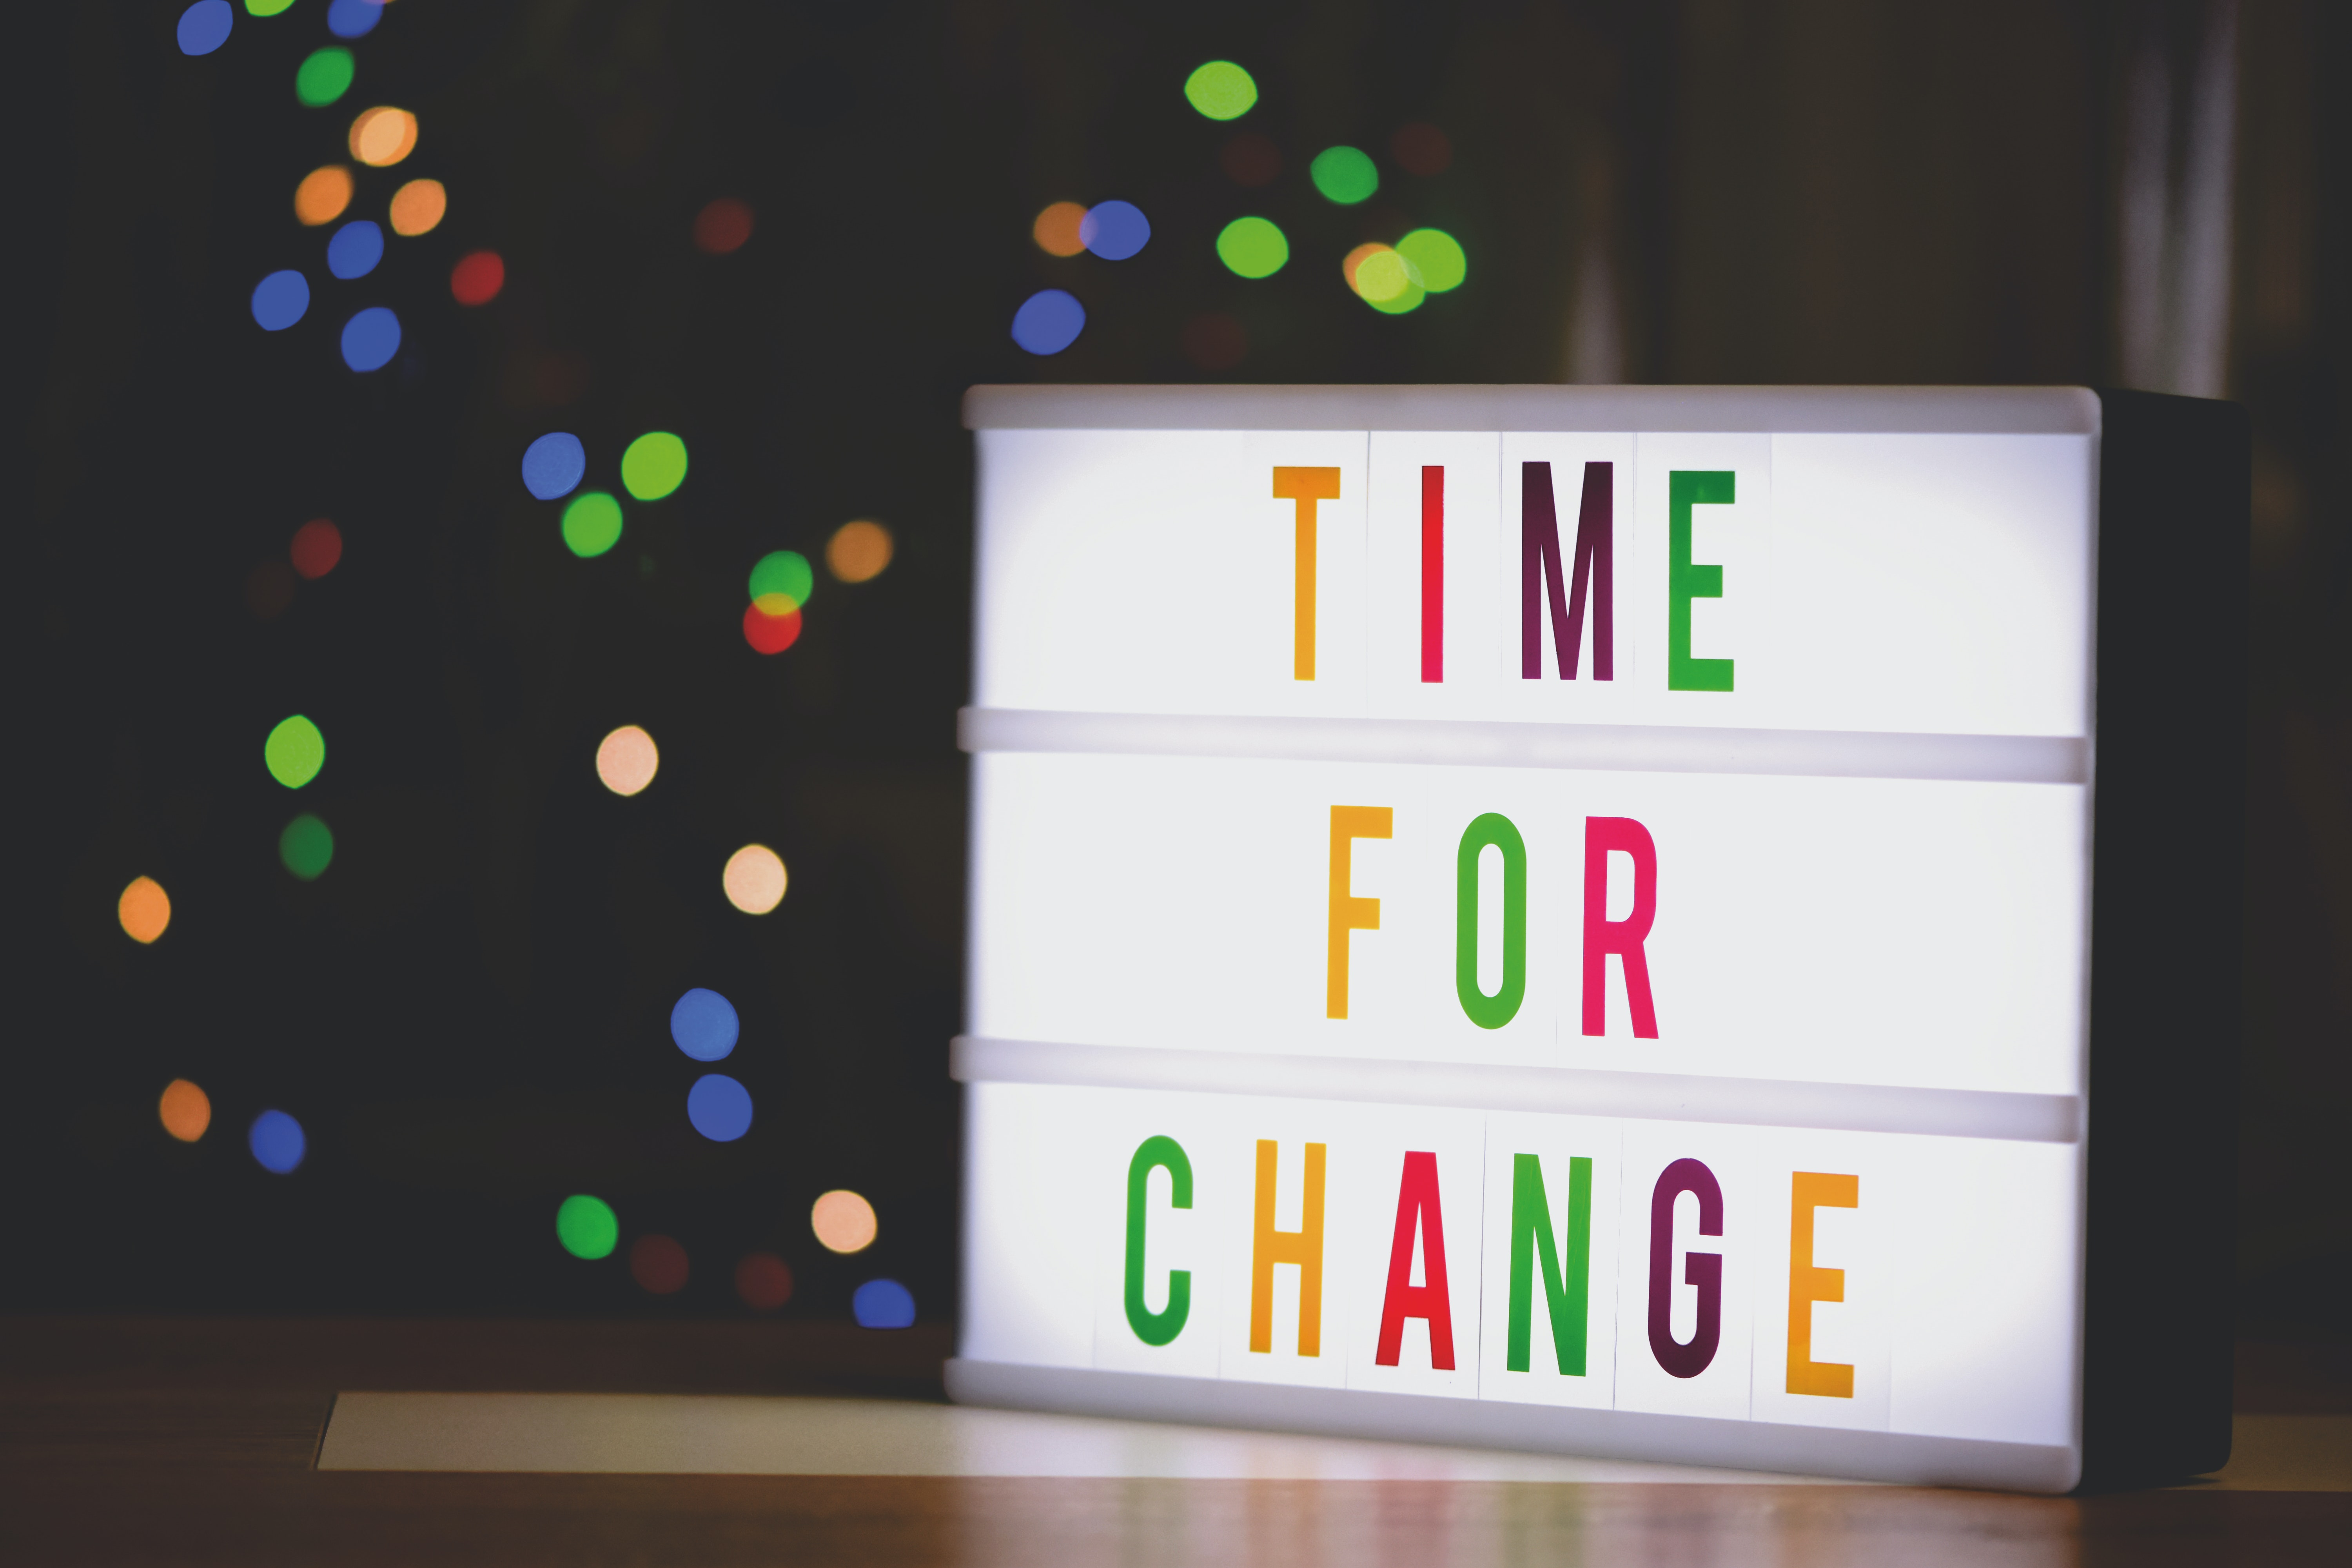
\includegraphics{somePicture}}
\advisor{Prof. Dr. Andreas Danuser}
\projectpartner{Rolf Lüscher}
\expert{Rolf Lüscher}
\degreeprogram{Bachelor of Science in Computer Science}
\setupSignature{
	Nicolo Lüscher={\includegraphics[width=.5\linewidth]{signature_nicolo_lüscher.png}}
}


%----------------  BFH tile page   -----------------------------------------
\maketitle
%------------ ABSTRACT        ----------------
\addchap{Abstract}
\section*{Abstract}

Abstract

%------------ TABLEOFCONTENTS ----------------
\tableofcontents

%------------ START MAIN PART ------------
\mainmatter

\chapter{First Thesis Chapter}
\chapter{Introduction}

\section{Motivation}
A family member of mine approached me with the request of looking into ways to monitor their beehives. They wanted to collect some basic information about their colonies like weight and temperature. This information should be made available over the internet and should be displayed in an easy-to-read format. The goal was to have an overview over the colonies and to be able to react to changes.

After listening to the request of my family member, I decided to look at the solutions that are commercially available. These are quite expensive, proprietary and not open source. Most of them also required a subscription from the manufacturer to work. I decided to look into the possibility of building my own solution. This would allow me to have a solution that is tailored to my needs and is open source.

This project was realized in the context of my Project 2 course at the Berne University of Applied Sciences.

\newpage
\section{Method}
Given that I was the only one working on this project, I decided to use a simple \gls{agile} development process. This process did not follow any classical agile methodology, but rather a simplified version of \gls{Kanban}. The process consisted of me defining a set of tasks that needed to be done. These tasks were then put into a \gls{backlog}. I then picked a task from the backlog and started working on it. Once the task was completed, I moved onto the next one. This process was repeated until the project was completed.
The tasks were grouped into a set of categories.

\subsection{Phases}

\subsubsection{Planning}
\textbf{Task: Research existing solutions}
\begin{itemize}
    \item Research existing solutions.
    \item Compare existing solutions.
    \item Analyze features of existing solutions.
\end{itemize}

\textbf{Task: Define requirements}
\begin{itemize}
    \item Define functional requirements.
    \item Define non-functional requirements.
    \item Discuss requirements with family member.
\end{itemize}

\textbf{Task: Rough Hardware Planning}
\begin{itemize}
    \item Define overall setup in regard to the functional requirements.
    \item Define components.
    \item Define communication protocols.
\end{itemize}

\textbf{Task: Specific Hardware Planning}
\begin{itemize}
    \item Define specific components.
    \item Define physical setup.
    \item Define wiring.
\end{itemize}

\newpage
\textbf{Task: Software Planning}
\begin{itemize}
    \item Define software stack.
    \item Define software architecture.
    \item Define data format.
    \item Define communication protocols.
    \item Define data flow.
    \item Define user interface.
\end{itemize}

\subsubsection{Implementation}
\textbf{Task: Build Prototype}
\begin{itemize}
    \item Procure components.
    \item Cut raw materials.
    \item Assemble prototype.
    \item Solder components.
    \item Test Components.
\end{itemize}

\textbf{Task: Server Setup}
\begin{itemize}
    \item Setup Docker environment.
    \item Setup MQTT broker.
    \item Setup PostgreSQL database.
    \item Setup NodeJS server.
    \item Integrate Express into NodeJS server.
    \item Integrate SequelizeJS into NodeJS server.
    \item Create database models.
    \item Persist MQTT messages into database.
    \item Create API routing.
    \item Create API endpoints.
\end{itemize}

\newpage
\textbf{Task: User Interface Setup}
\begin{itemize}
    \item Setup Angular environment.
    \item Integrate Tailwind CSS into Angular.
    \item Integrate ChartJS into Angular.
    \item Create basic layout.
    \item Create data service.
    \item Visualize data with ChartJS.
\end{itemize}

\subsubsection{Testing}
\textbf{Task: Test Setup}
\begin{itemize}
    \item Setup test environment.
    \item Test weight sensor.
    \item Test weight calibration.
    \item Test temperature sensor.
    \item Test power consumption.
    \item Test user interface.
    \item Test end to end communication.
\end{itemize}

\subsubsection{Documentation}
\textbf{Task: Documentation}
\begin{itemize}
    \item Setup LaTeX environment.
    \item Write documentation.
\end{itemize}
\section{Methods}
What did you do? – a section which details how the research was performed.  It typically features a description of the participants/subjects that were involved, the study design, the materials that were used, and the study procedure.  If there were multiple experiments, then each experiment may require a separate Methods section.  A rule of thumb is that the Methods section should be sufficiently detailed for another researcher to duplicate your research.

\chapter{Results}
\section{System}
During the building process it became more and more clear that this project would be more of a proof of concept other than a fully fetched, commercially viable product. There are just too many factors and variables that need to be considered in building a long-lasting, reliable, off-the-grid, weatherproof, accurate measuring system. For this reason, the system was more of a proof of concept than a fully fledged product and still needs some improvements to be made before it can be used in a real-world scenario.

Nonetheless, the resulting system fulfilled most of the requirements outlined in the planning phase and provides a solid base to be improved upon in the future. It fulfills its core functionality goals of collecting measurements of a beehive in a remote location and transmitting them to a central server where it can be accessed by a user interface. 

\begin{figure}
    \centering
    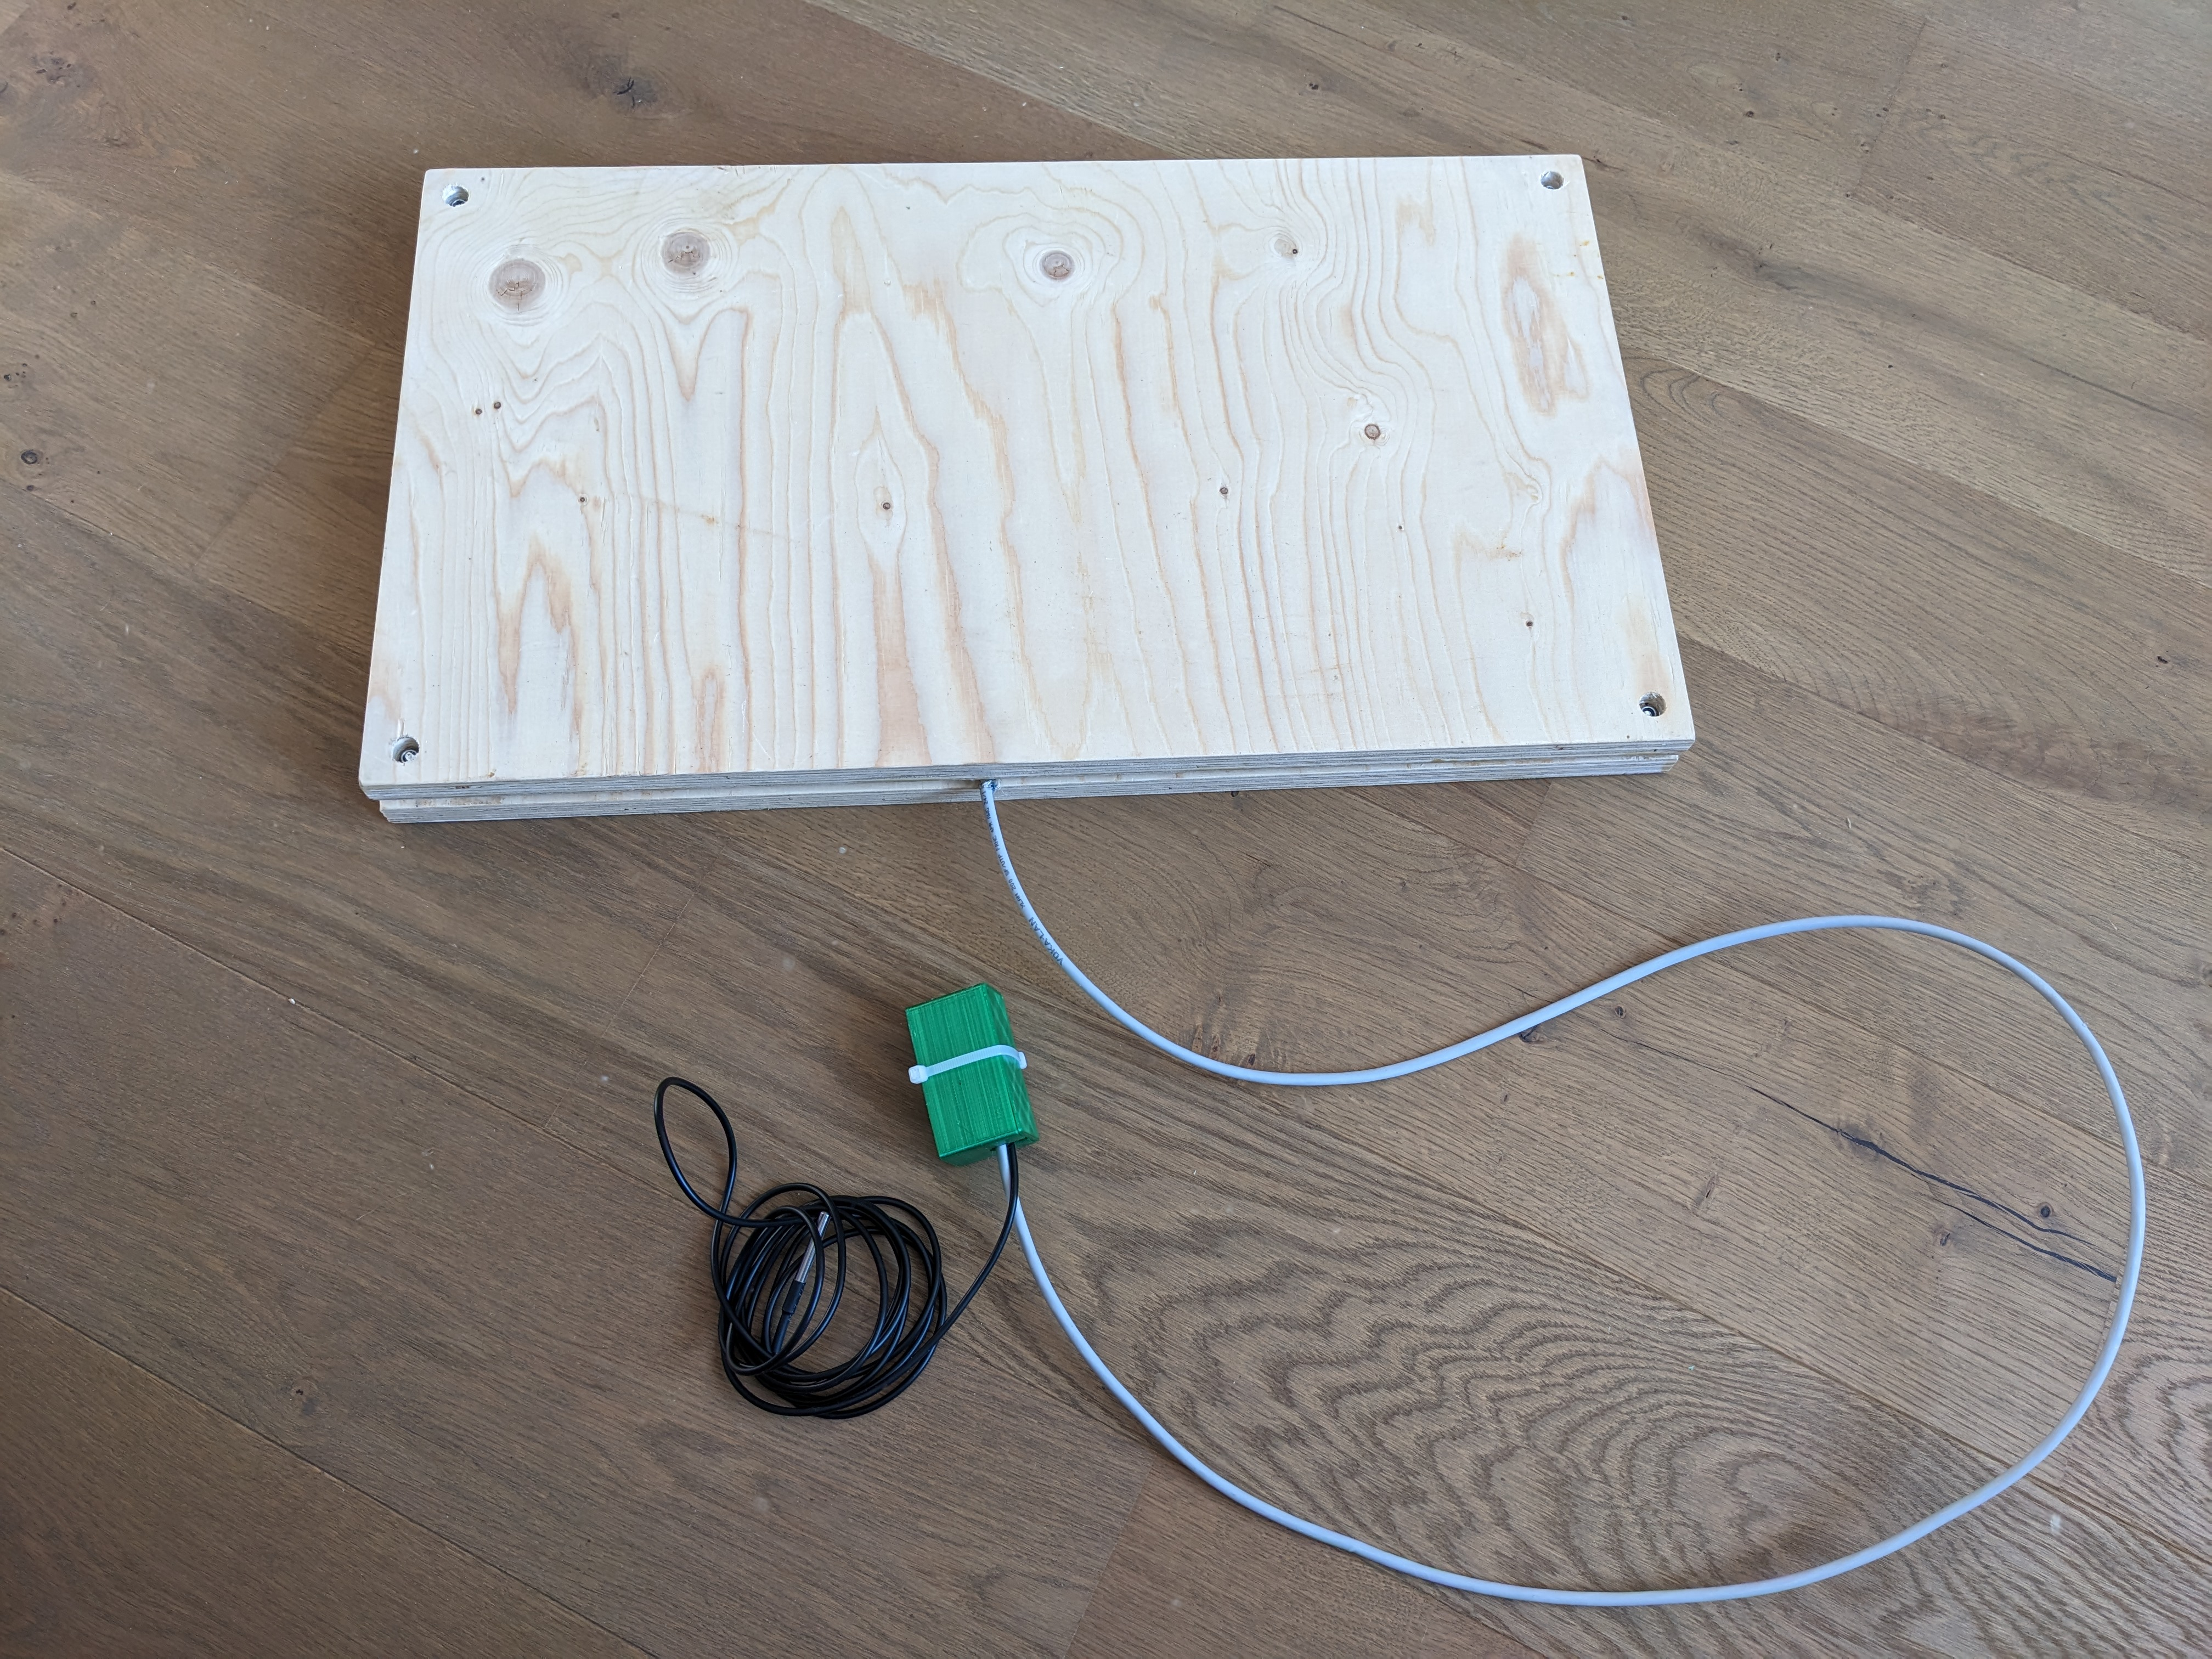
\includegraphics[width=0.55\textwidth]{figures/scale.jpg}
    \caption{Overview of the system}
    \label{fig:overview}
\end{figure}

\begin{figure}
    \centering
    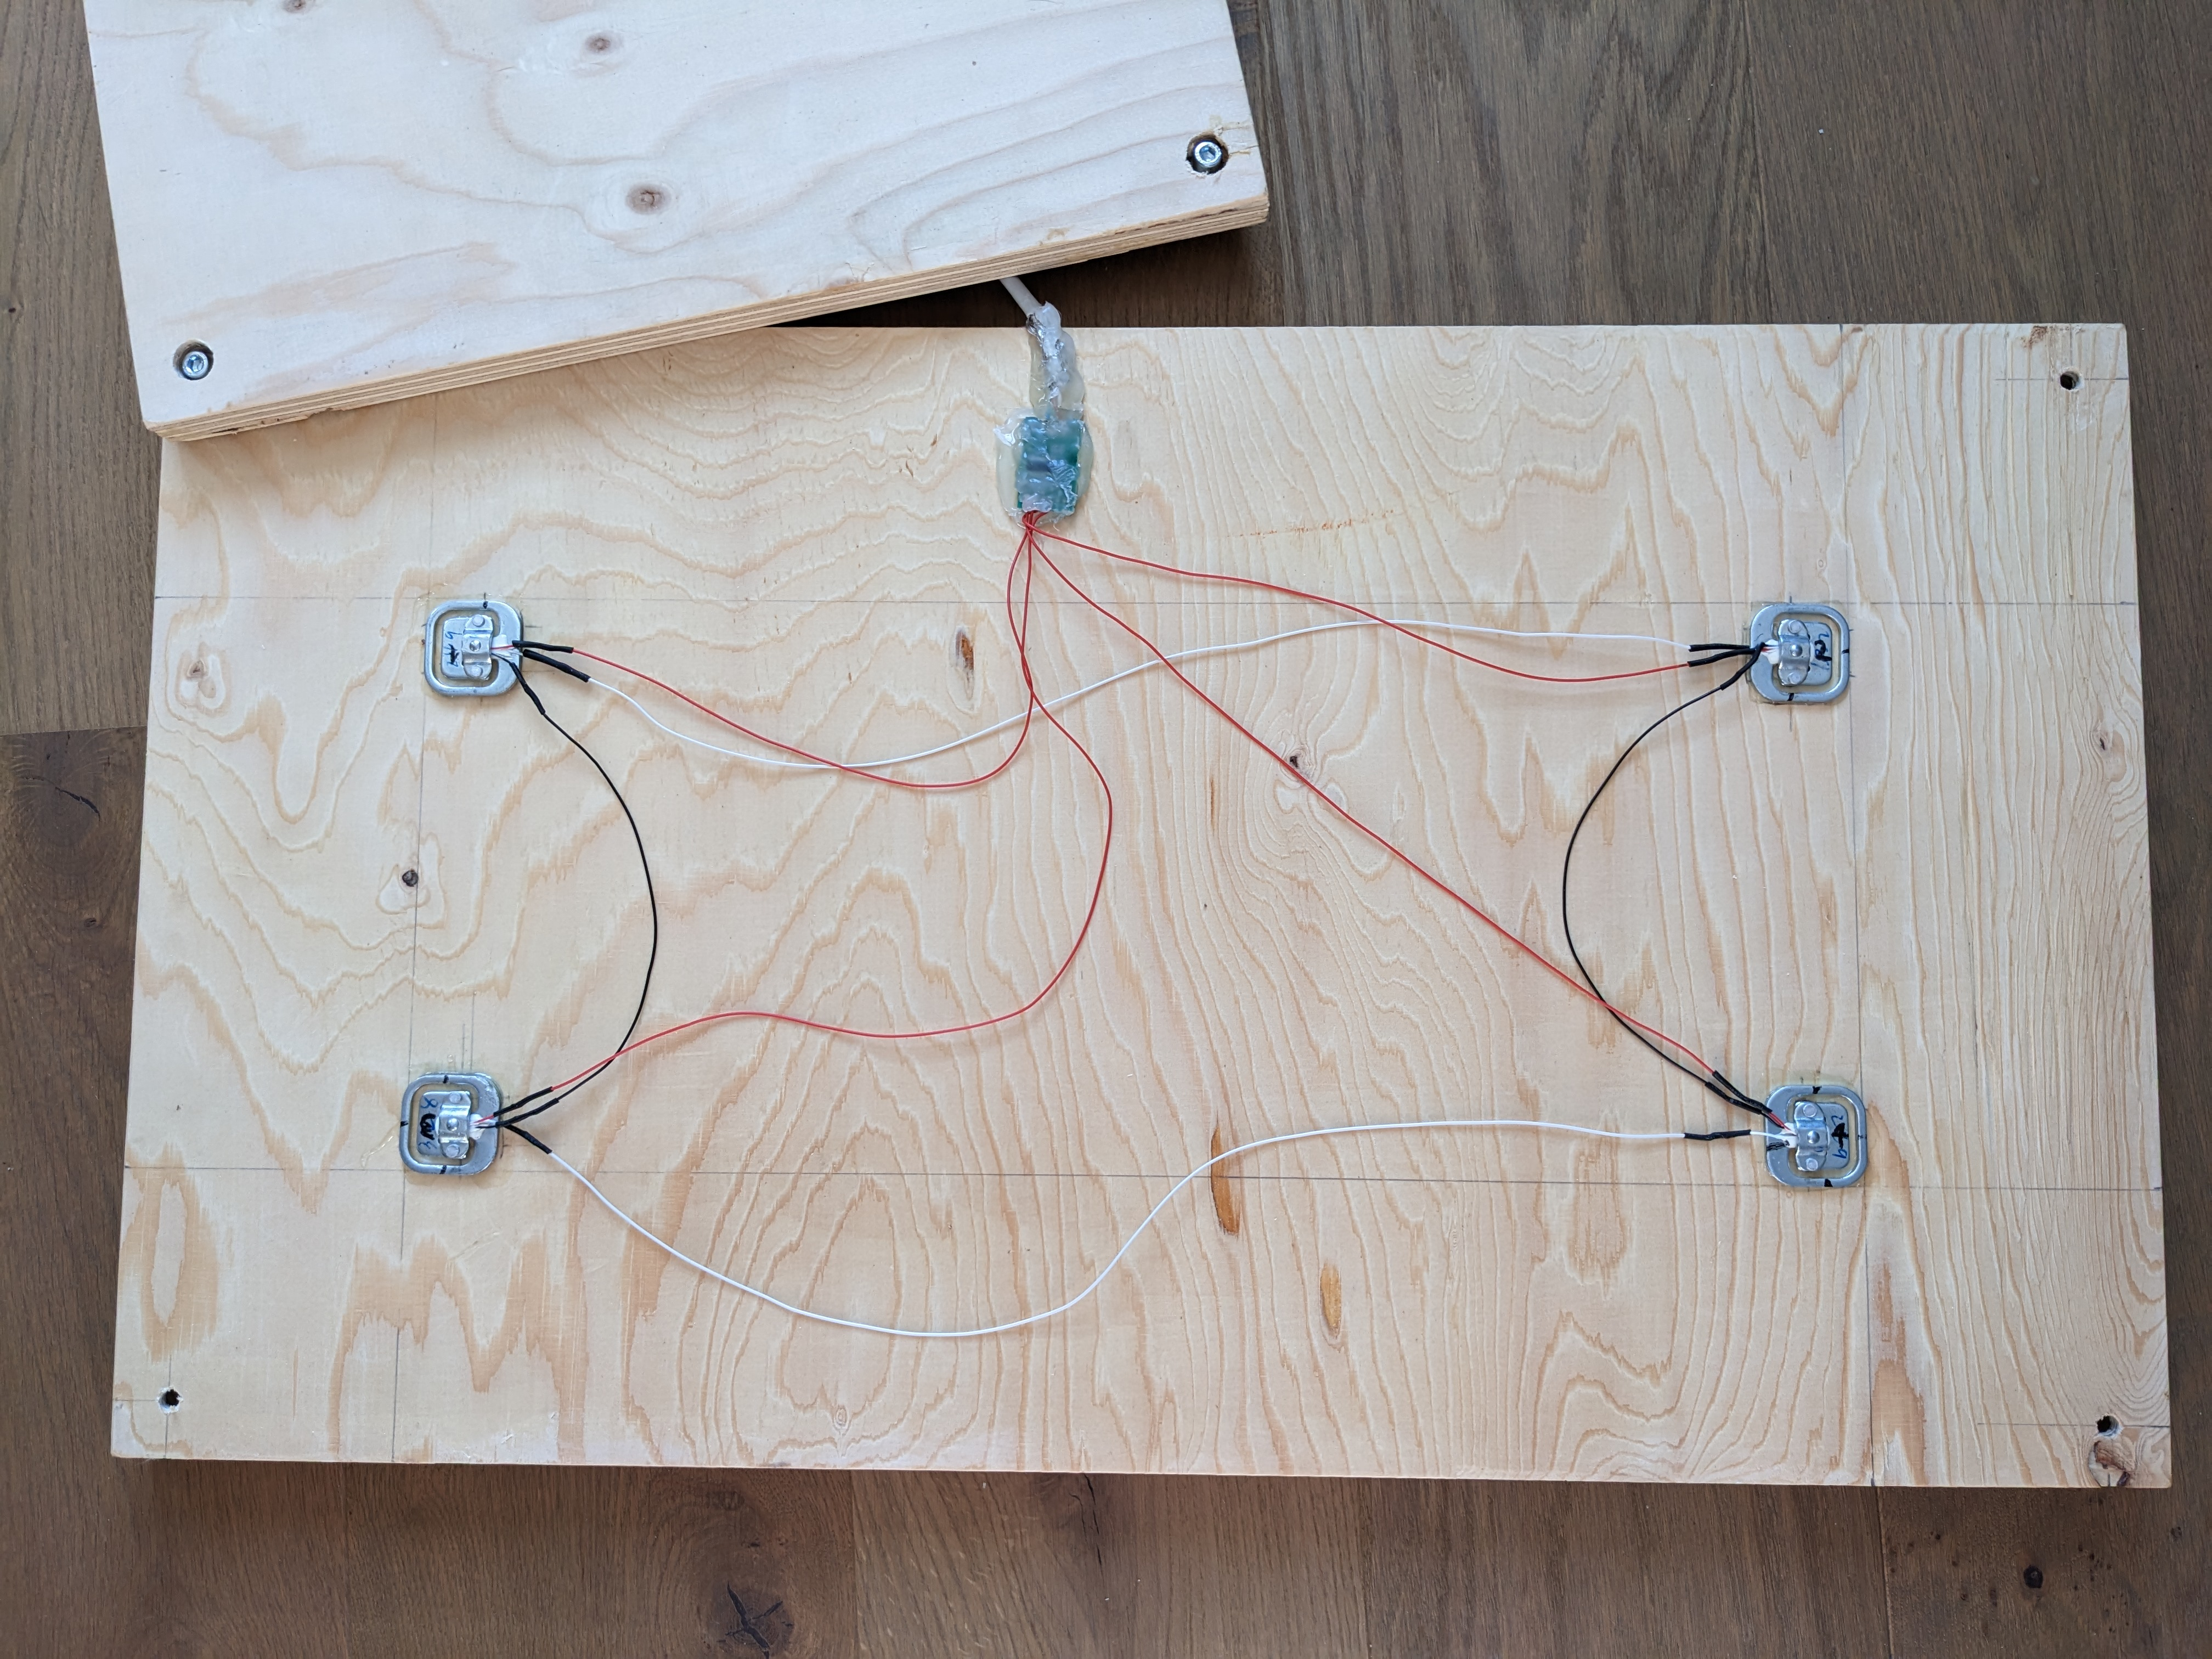
\includegraphics[width=0.55\textwidth]{figures/scale_wiring.jpg}
    \caption{Internal wiring of the scale}
    \label{fig:overview}
\end{figure}

\begin{figure}
    \centering
    \includegraphics[width=0.55\textwidth]{figures/esp32_connected.jpg}
    \caption{Internal wiring of the microcontroller}
    \label{fig:overview}
\end{figure}

\newpage
\newpage
\section{Costs}
The main goal of this project was to build the system as cost-effective as possible. The following table shows the total cost it took to build the system.

\begin{table}[ht]
    \centering
    \begin{bfhTabular}{llll}
       Name & Quantity & Price & Total
       \\\hline
       Wood & \num{1} & CHF\num{41.00} & CHF\num{41.00}\\\hline
       Wood Treatment & \num{1} & CHF\num{3.00} & CHF\num{3.00}\\\hline
       Cables & \num{1} & CHF\num{3.00} & CHF\num{3.00}\\\hline
       Temperature Sensor (DS18B20) & \num{1} & CHF\num{10.90} & CHF\num{10.90}\\\hline
       18650 LiPo Battery & \num{4} & CHF\num{8.90} & CHF\num{35.60}\\\hline
       LiPo Battery 4x Shield & \num{1} & CHF\num{16.90} & CHF\num{16.90}\\\hline
       Generic Load Cell & \num{4} & CHF\num{4.50} & CHF\num{18.00}\\\hline
       HX711 Load Cell Amplifier & \num{1} & CHF\num{4.50} & CHF\num{4.50}\\\hline
       LILYGO TTGO T-Call ESP32 SIM800L & \num{1} & CHF\num{25.17} & CHF\num{25.17}\\\hline
       Misc. Nuts, Bolts and other consumables & \num{1} & CHF\num{10.00} & CHF\num{10.00}\\\hline
       Data Plan for 365 Days & \num{1} & CHF\num{44.00} & CHF\num{44.00}\\\hline
        &  & \textbf{Total} & \textbf{CHF212.07}\\\hline
    \end{bfhTabular}
    \caption{Price of the system}
    \label{tab:tab1}
 \end{table}

This is way cheaper that even the cheaper commercially available beehive monitoring systems with the added benefit of being completely open source and customizable. This price doesn't include the time it took to build the system, which is a significant factor in the total cost of the system. Most of the time however was spent on the design, planning and research phase, which wouldn't need to be done again  for future iterations of the system.

 \newpage
\section{Conclusion}
\subsection{Future Improvements}
The system as it is right now is not really usable in the way it was intended. There are still some major improvements that need to be done like changing the material of the scale to something less subjectable to thermal expansion and addressing the load cell inaccuracies. Another important aspect is creating a weatherproof housing for the microcontroller and the batteries.

Another important aspect is providing solar power to the batteries. This would reduce the need for frequent battery changes and would make the system more reliable.

More user interfaces like SMS/Email notifications would also be a nice addition to the system.

Another interesting future prospect would be the addition of data analysis to the system. This would allow the user to get a better understanding of the data collected by the system and would allow for better decision-making. There could also be systems to make predictions about the future based on the data collected. For example a prediction of when the honey will be ready to harvest and how much the expected yield will be. Another system would be the prediction and detection of a swarm. This would allow the user to take action before the swarm leaves the hive and would allow for better swarm management.

\newpage
\subsection{Reflection}
All in all I think this project was a success. I was able to come up with a setup that did what it was supposed to do. Furthermore, I have learned a lot about designing and building IOT projects and the technologies used in the project. I am looking forward to improving the system in the future and transform it into a completely viable product. It is also my intention to make the system open source and share it with the community.

During the project, I've encountered some quite significant roadblocks, that I was able to overcome. I believe that this greatly improved my problem-solving skills and my ability to work under pressure. A lot of the problems I encountered were in fields I had no experiences in, which made it even more challenging. But I believe that solving those issues and thinking about the problems that arose made me a better engineer.

In conclusion, I really enjoyed working on this project, and I am looking forward to start working on my bachelor thesis.


\chapter{Second Thesis Chapter}
\section{Some \texorpdfstring{\LaTeX}{LaTeX}~Examples}

\blindtext[1]

\subsection{Tabular}

\begin{tabular}[h]{l|l|l}
  \centering
	Measure & Data & Unit \\ \hline
	1      & 2	  & 3  \\
	4      & 5	  & 6
\end{tabular}

% Example for a Table in BFH-Style with a simple Design
\begin{table}[ht]
   \centering
   \begin{bfhTabular}{lll}
      Stadtteil & Anzahl Personen & Ausländische
      Bevölkerung\\\hline
      Innere Stadt & \num{3748} & \SI{17.9}{\percent}\\\hline
      Länggasse-Felsenau & \num{17976} & \SI{17.1}{\percent}\\\hline
      Mattenhof-Weissenbühl & \num{26895} & \SI{22.4}{\percent}\\\hline
      Kirchenfeld-Schlosshalde & \num{23384} & \SI{13.4}{\percent}\\\hline
      Breitenrain-Lorraine & \num{24082} & \SI{19.4}{\percent}
   \end{bfhTabular}
   \caption{Anzahl Personen, ausländischer Bevölkerungsanteil und Arbeitslosenquote pro
	Stadtteil Ende 2005 (Statistikdienste der Stadt Bern, 2006)}
   \label{tab:tab1}
\end{table}

\begin{table}[ht]
   \centering
   \colorlet{BFH-table}{BFH-MediumBlue!10}
   \colorlet{BFH-tablehead}{BFH-MediumBlue!50}
   \begin{bfhTabular}{lll}
      Stadtteil & Anzahl Personen & Ausländische
      Bevölkerung\\\hline
      Innere Stadt & \num{3748} & \SI{17.9}{\percent}\\\hline
      Länggasse-Felsenau & \num{17976} & \SI{17.1}{\percent}\\\hline
      Mattenhof-Weissenbühl & \num{26895} & \SI{22.4}{\percent}\\\hline
      Kirchenfeld-Schlosshalde & \num{23384} & \SI{13.4}{\percent}\\\hline
      Breitenrain-Lorraine & \num{24082} & \SI{19.4}{\percent}
   \end{bfhTabular}
   \caption{Anzahl Personen, ausländischer Bevölkerungsanteil und Arbeitslosenquote pro
	Stadtteil Ende 2005 (Statistikdienste der Stadt Bern, 2006)}
   \label{tab:tab2}
\end{table}

\begin{table}[ht]
   \centering
   \colorlet{BFH-table}{BFH-MediumRed!10}
   \colorlet{BFH-tablehead}{BFH-MediumRed!50}
   \begin{bfhTabular}{lll}
      Stadtteil & Anzahl Personen & Ausländische
      Bevölkerung\\\hline
      Innere Stadt & \num{3748} & \SI{17.9}{\percent}\\\hline
      Länggasse-Felsenau & \num{17976} & \SI{17.1}{\percent}\\\hline
      Mattenhof-Weissenbühl & \num{26895} & \SI{22.4}{\percent}\\\hline
      Kirchenfeld-Schlosshalde & \num{23384} & \SI{13.4}{\percent}\\\hline
      Breitenrain-Lorraine & \num{24082} & \SI{19.4}{\percent}
   \end{bfhTabular}
   \caption{Anzahl Personen, ausländischer Bevölkerungsanteil und Arbeitslosenquote pro
	Stadtteil Ende 2005 (Statistikdienste der Stadt Bern, 2006)}
   \label{tab:tab3}
\end{table}


\begin{description}
\item[More about Tables] Further information about tables : \url{https://www.latex-tutorial.com/tutorials/tables/}
\item[Long Tables] Further information about long tables : \url{https://www.overleaf.com/learn/latex/tables}
\end{description}


\begin{longtable}{|l|l|l|}
\caption{A sample long table} \label{tab:long} \\


\hline \multicolumn{1}{|c|}{\textbf{First column}} & \multicolumn{1}{c|}{\textbf{Second column}} & \multicolumn{1}{c|}{\textbf{Third column}} \\ \hline 
\endfirsthead

\multicolumn{3}{c}%
{{\tablename\ \thetable{}: \hfill $...$~continued from previous page}} \\
\hline \multicolumn{1}{|c|}{\textbf{First column}} & \multicolumn{1}{c|}{\textbf{Second column}} & \multicolumn{1}{c|}{\textbf{Third column}} \\ \hline 
\endhead

\hline \multicolumn{3}{|r|}{{Continued on next page$...$}} \\ \hline
\endfoot

\hline \hline
\endlastfoot
\centering

One & abcdef ghjijklmn & 123.456778 \\
One & abcdef ghjijklmn & 123.456778 \\
One & abcdef ghjijklmn & 123.456778 \\
One & abcdef ghjijklmn & 123.456778 \\
One & abcdef ghjijklmn & 123.456778 \\
One & abcdef ghjijklmn & 123.456778 \\
One & abcdef ghjijklmn & 123.456778 \\
One & abcdef ghjijklmn & 123.456778 \\
One & abcdef ghjijklmn & 123.456778 \\
One & abcdef ghjijklmn & 123.456778 \\
One & abcdef ghjijklmn & 123.456778 \\
One & abcdef ghjijklmn & 123.456778 \\
One & abcdef ghjijklmn & 123.456778 \\
One & abcdef ghjijklmn & 123.456778 \\
One & abcdef ghjijklmn & 123.456778 \\
One & abcdef ghjijklmn & 123.456778 \\
One & abcdef ghjijklmn & 123.456778 \\
One & abcdef ghjijklmn & 123.456778 \\
One & abcdef ghjijklmn & 123.456778 \\
One & abcdef ghjijklmn & 123.456778 \\
One & abcdef ghjijklmn & 123.456778 \\
One & abcdef ghjijklmn & 123.456778 \\
One & abcdef ghjijklmn & 123.456778 \\
One & abcdef ghjijklmn & 123.456778 \\
One & abcdef ghjijklmn & 123.456778 \\
One & abcdef ghjijklmn & 123.456778 \\
One & abcdef ghjijklmn & 123.456778 \\
One & abcdef ghjijklmn & 123.456778 \\
One & abcdef ghjijklmn & 123.456778 \\
One & abcdef ghjijklmn & 123.456778 \\
One & abcdef ghjijklmn & 123.456778 \\
One & abcdef ghjijklmn & 123.456778 \\
One & abcdef ghjijklmn & 123.456778 \\
One & abcdef ghjijklmn & 123.456778 \\
One & abcdef ghjijklmn & 123.456778 \\
One & abcdef ghjijklmn & 123.456778 \\
One & abcdef ghjijklmn & 123.456778 \\
One & abcdef ghjijklmn & 123.456778 \\
One & abcdef ghjijklmn & 123.456778 \\
One & abcdef ghjijklmn & 123.456778 \\
One & abcdef ghjijklmn & 123.456778 \\
One & abcdef ghjijklmn & 123.456778 \\
One & abcdef ghjijklmn & 123.456778 \\
One & abcdef ghjijklmn & 123.456778 \\
One & abcdef ghjijklmn & 123.456778 \\
One & abcdef ghjijklmn & 123.456778 \\
One & abcdef ghjijklmn & 123.456778 \\
One & abcdef ghjijklmn & 123.456778 \\
One & abcdef ghjijklmn & 123.456778 \\
One & abcdef ghjijklmn & 123.456778 \\
One & abcdef ghjijklmn & 123.456778 \\
One & abcdef ghjijklmn & 123.456778 \\
One & abcdef ghjijklmn & 123.456778 \\
One & abcdef ghjijklmn & 123.456778 \\
One & abcdef ghjijklmn & 123.456778 \\
One & abcdef ghjijklmn & 123.456778 \\
One & abcdef ghjijklmn & 123.456778 \\
One & abcdef ghjijklmn & 123.456778 \\
One & abcdef ghjijklmn & 123.456778 \\
One & abcdef ghjijklmn & 123.456778 \\
One & abcdef ghjijklmn & 123.456778 \\
One & abcdef ghjijklmn & 123.456778 \\
One & abcdef ghjijklmn & 123.456778 \\
One & abcdef ghjijklmn & 123.456778 \\
One & abcdef ghjijklmn & 123.456778 \\
One & abcdef ghjijklmn & 123.456778 \\
One & abcdef ghjijklmn & 123.456778 \\
One & abcdef ghjijklmn & 123.456778 \\
One & abcdef ghjijklmn & 123.456778 \\
One & abcdef ghjijklmn & 123.456778 \\
One & abcdef ghjijklmn & 123.456778 \\
One & abcdef ghjijklmn & 123.456778 \\
One & abcdef ghjijklmn & 123.456778 \\
One & abcdef ghjijklmn & 123.456778 \\
One & abcdef ghjijklmn & 123.456778 \\
\end{longtable}
 

\subsection{Math}
%% Mathematical equations
\begin{align}
\left(\begin{array}{r}
\dot{x_{1}} \\                                              
\dot{x_{2}} \\ 
\dot{x_{3}} \\                                 
\end{array}\right) =
\left[\begin{array}{rrr}
0 & 1 & 0 \\                                              
0 & -\frac{b_{f}}{J} & \frac{K_{m}}{J} \\
0 & -\frac{K_{g}}{L} & \frac{R}{L} \\                                      
\end{array}\right]
\left(\begin{array}{r}
x_{1} \\                                              
x_{2} \\ 
x_{3} \\                                 
\end{array}\right) +
\left[\begin{array}{rr}
0 & 0 \\                                              
-\frac{1}{J} & 0 \\ 
0 & \frac{1}{L} \\                                 
\end{array}\right]
\left(\begin{array}{r}
t_{L} \\                                              
v_{a} \\                                 
\end{array}\right)
\end{align}

\subsection{Include pictures}

\begin{figure}[H]
  \centering
  
\includegraphics[width=.8\textwidth]{placeholder}
  \caption{Some meaningful caption}
  \label{fig:placeholder:1}
\end{figure}


\begin{figure}[h!]
  \centering
  \begin{minipage}{.4\textwidth}
  	\centering
	
\includegraphics[width=\textwidth]{placeholder}
	\caption{PLACEHOLDER}
	\label{fig:placeholder:2}
  \end{minipage}
  \hspace{1em}
  \begin{minipage}{.4\textwidth}
	\centering
	
\includegraphics[width=\textwidth]{placeholder}
	\caption{PLACEHOLDER}
	\label{fig:placeholder:3}
  \end{minipage}%
\end{figure}


%% Source code is stored in the listings folder and will be included from there using its relative path.
\subsection{Code Example}

{
  \thicklines
% \thinlines
\lstinputlisting[style=bfh-c,language=C,caption={My very first C program.},label={lst:hello}]{listings/expl_hello.c}
}
I developed this very nice application writing "Hello World" to my terminal.
The implementation is shown in listing~\ref{lst:hello}.


%% Examples holding dummy content
\subsection{Draw boxes}
\begin{bfhBox}[BFH-DarkPurple]{Purple}
	Note\\
\end{bfhBox}

\blindtext[1]

\begin{bfhBox}[BFH-MediumBlue]{Blue}
	Note\\
\end{bfhBox}

\blindtext[1]

\begin{bfhBox}[BFH-DarkRed]{Red}
	Note\\
\end{bfhBox}

\blindtext[2]

\begin{bfhAlertBox}
  An alert box.
\end{bfhAlertBox}

\begin{bfhWarnBox}
  A warning box.
\end{bfhWarnBox}

\begin{bfhNoteBox}
  A note box.
\end{bfhNoteBox}

\begin{bfhRecycleBox}
  A recycle box.
\end{bfhRecycleBox}


\begin{bfhBox}{No color set}
	Some BFH box without color option set. Using default.\\
\end{bfhBox}


\blindtext[3]


\subsection{Some Item-list}
Sometimes you explain this and that using a bullet points.
This can be done in \LaTeX\ using an item list in a item environment.

\begin{itemize}
\item My first item
\item The second
\item $\cdots$
\item $\cdots$
\end{itemize}

It is also possible to nest such environment and/or enumerate.
\begin{itemize}
\item My first item
\begin{enumerate}
\item My first enumerated item
\item The second
\item $\cdots$
\end{enumerate}
\item The second
\begin{enumerate}
\item An other enumerated item
\item $\cdots$
\item $\cdots$
\end{enumerate}
\end{itemize}


\subsection{Multi column environment}
Split a part of a document in multiple columns is not so easy with WYSIWYG tools.
Whit multicols \LaTeX\ package$\cdots$ well you may know.

\begin{multicols}{3}
\begin{itemize}
\item My first item
\item The second
\item $\cdots$
\item $\cdots$
\end{itemize}
\begin{itemize}
\item My first item
\item The second
\item $\cdots$
\item $\cdots$
\end{itemize}
\begin{itemize}
\item My first item
\item The second
\item $\cdots$
\item $\cdots$
\end{itemize}
\end{multicols}


\blindtext[1]

\begin{multicols}{2}
  \blindtext[1]
\end{multicols}

\begin{multicols}{3}
  \blindtext[1]
\end{multicols}

\begin{multicols}{2}
  \blindtext[1]
\end{multicols}


\begin{multicols}{3}
\begin{itemize}
\item My first item
\item The second
\item $\cdots$
\item $\cdots$
\end{itemize}
\blindtext[1]
\columnbreak
\begin{itemize}
\item My first item
\item The second
\item $\cdots$
\item $\cdots$
\end{itemize}
\end{multicols}

%% forced page break
\newpage

\subsection{Use Figures}

\begin{figure}[h!]
  \centering
  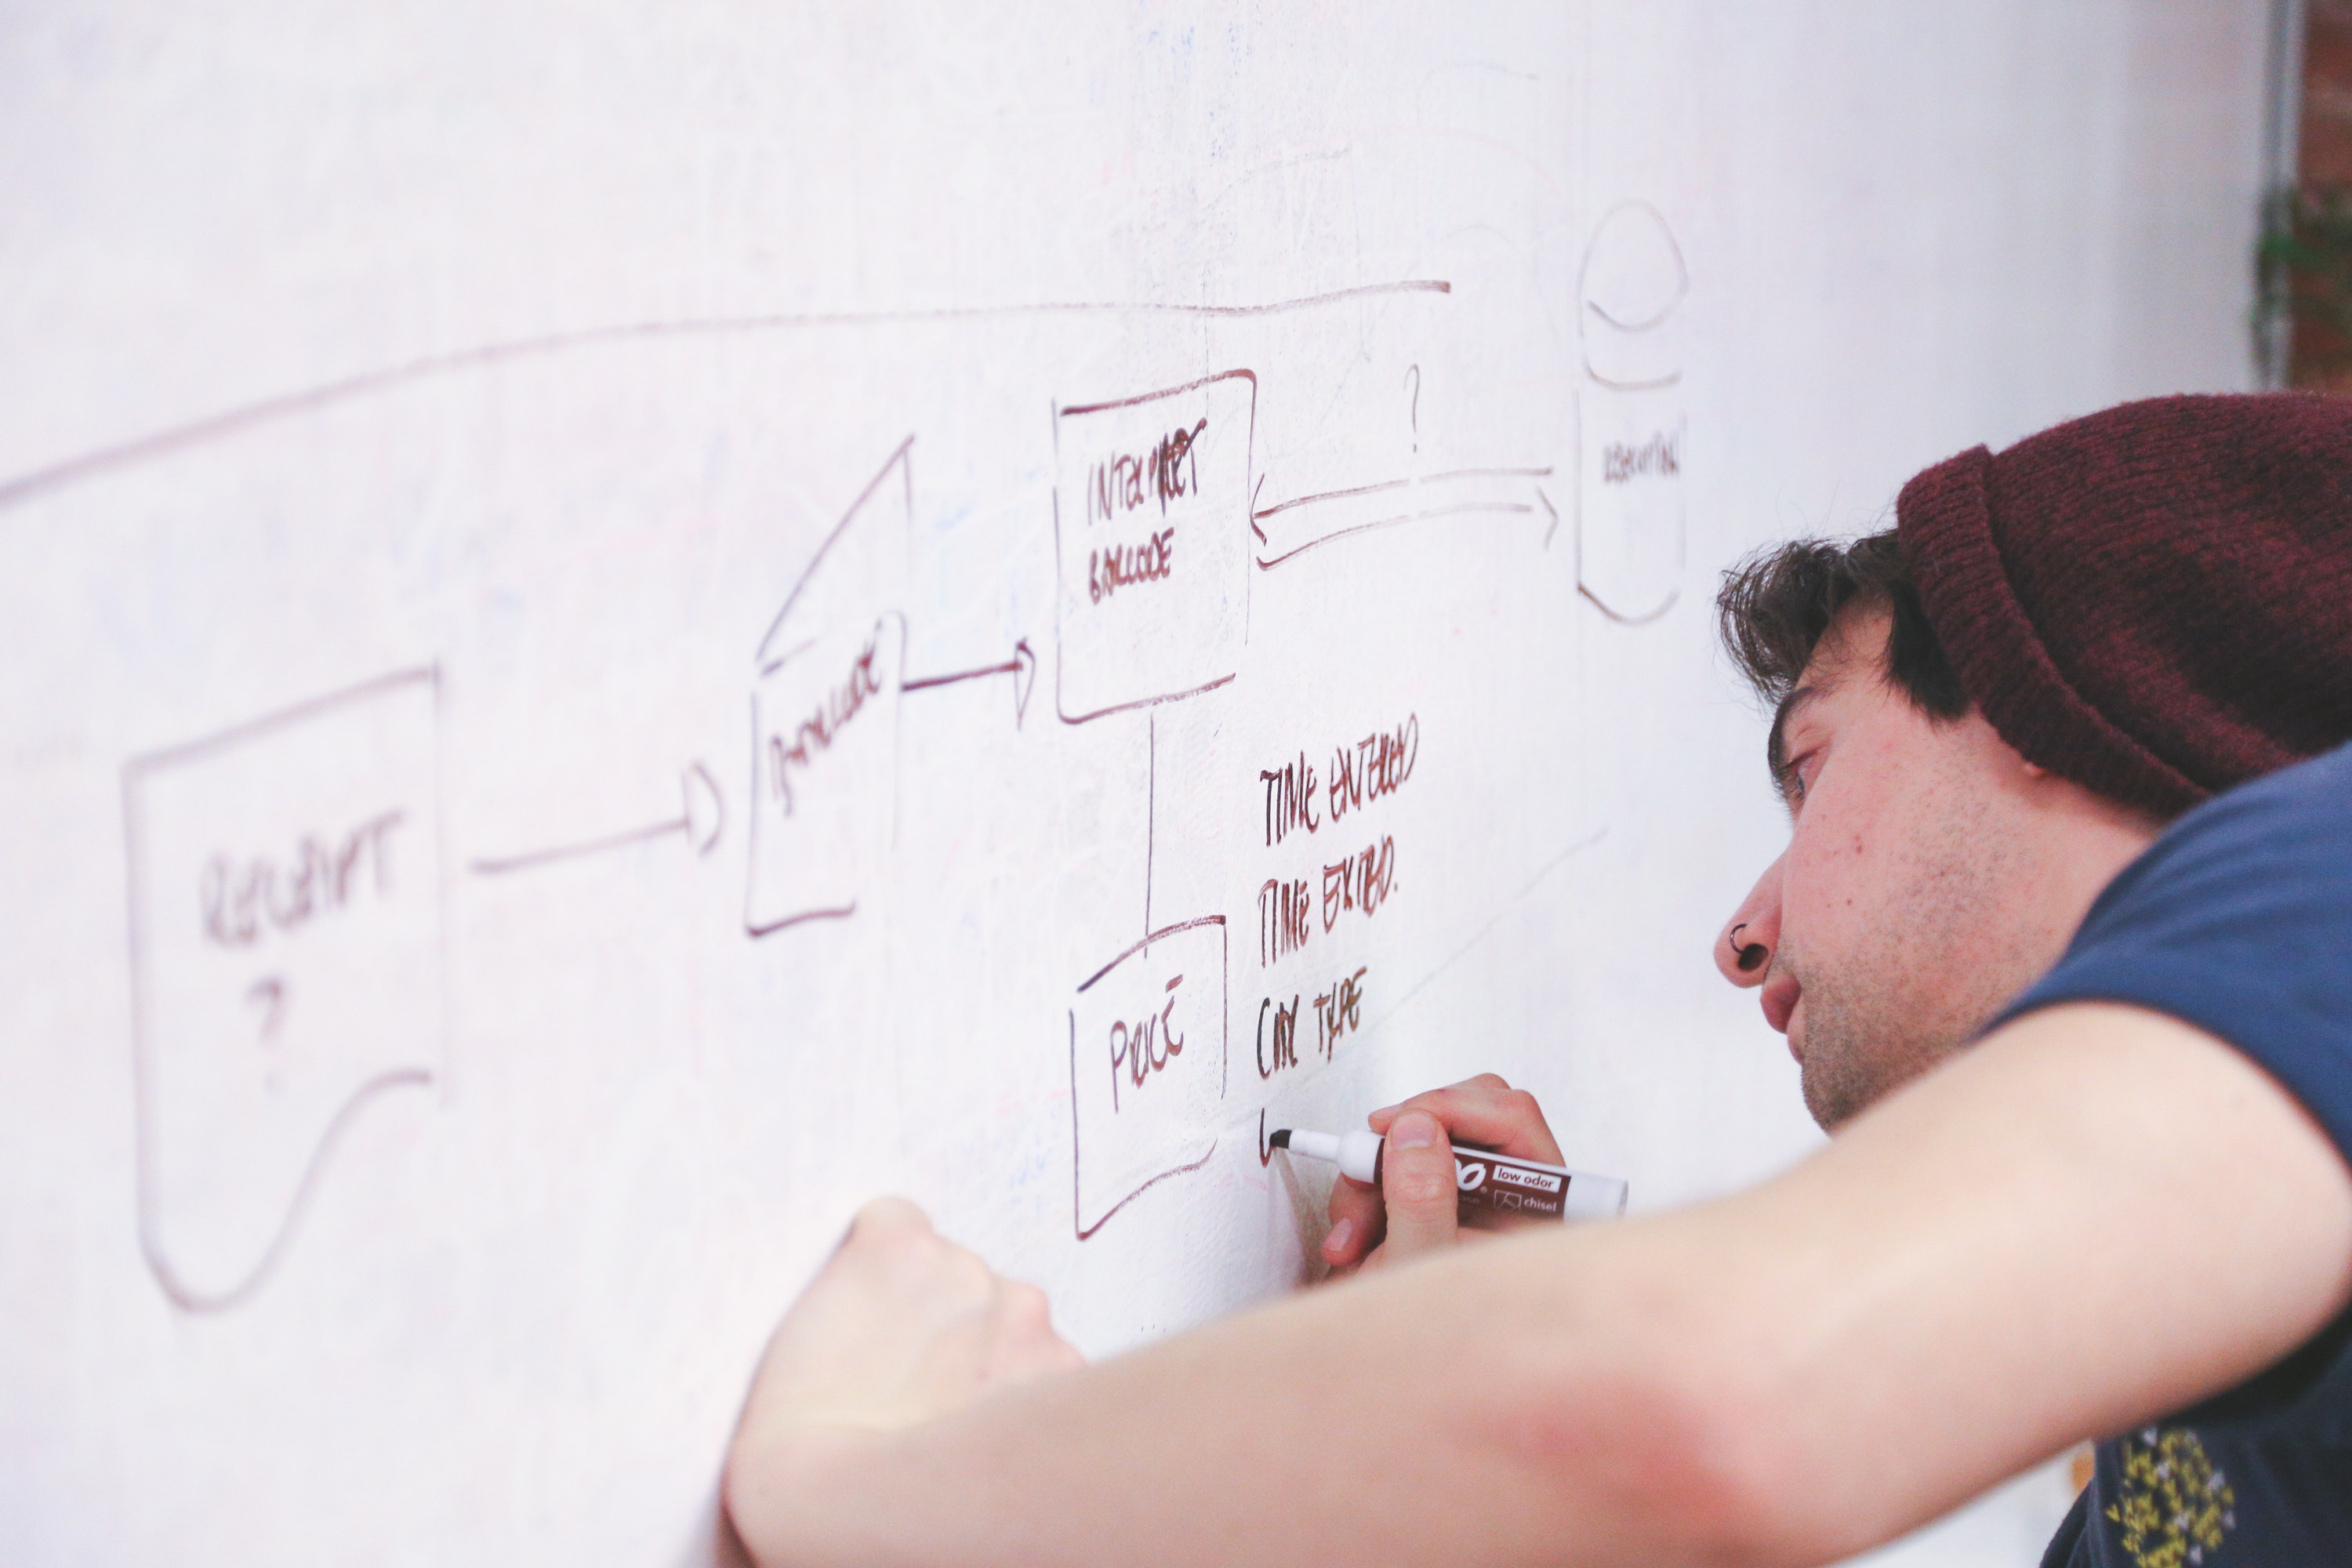
\includegraphics[width=.8\textwidth]{bg-masthead}
  \caption{An example of including a PDF figure.}
  \label{fig:expl_master}
\end{figure}

\begin{figure}[h!]
  \centering
  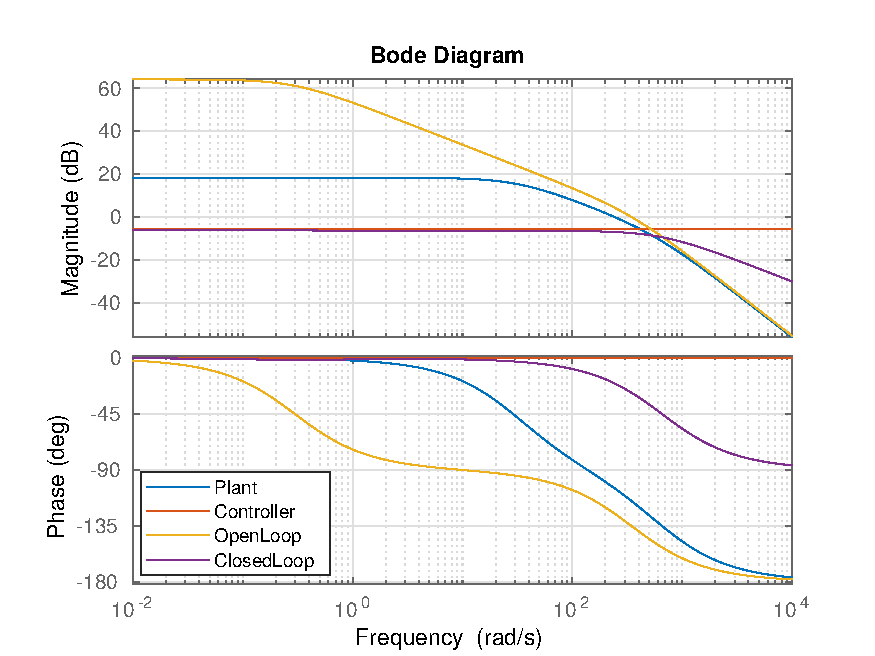
\includegraphics[width=.8\textwidth]{expl_bode}
  \caption{An example of including a PDF figure.}
  \label{fig:expl_bode}
\end{figure}
\clearpage

\subsubsection{Use Subfigures}
These subfigures requires the package \texttt{subcaption}.

\begin{figure}[h!]
     \centering
     \begin{subfigure}[b]{0.3\textwidth}
         \centering
         
\includegraphics[width=\textwidth]{placeholder}
         \caption{$y=x$}
         \label{fig:y equals x}
     \end{subfigure}
     \hfill
     \begin{subfigure}[b]{0.3\textwidth}
         \centering
         
\includegraphics[width=\textwidth]{placeholder}
         \caption{$y=3sinx$}
         \label{fig:three sin x}
     \end{subfigure}
     \hfill
     \begin{subfigure}[b]{0.3\textwidth}
         \centering
         
\includegraphics[width=\textwidth]{placeholder}
         \caption{$y=5/x$}
         \label{fig:five over x}
     \end{subfigure}
        \caption{Three simple graphs}
        \label{fig:three graphs}
\end{figure}


\section{Example Text With Indices}
In this example, several keywords\index{keywords} will be used 
which are important and deserve to appear in the Index\index{Index}.

Terms like generate\index{generate} and some\index{others} will 
also show up.

\section{Example Text With Glossary}
This \Gls{zynq} introduction summary has been written for bachelor students due to the introduction workshop in the ``Embedded Systems'' course at Bern University of Applied Sciences. The topic \Gls{soc} is introduced by using Xilinx' \Gls{apsoc} platform \Gls{zynq}. The subsequent summery is a brief introduction only. It is based on several tutorials in the field of \Gls{soc} such as the \Gls{zbook} or Xilinx' \Gls{apsoc} manual. We think the script provides a good introduction and helps getting the overall picture of the \Gls{soc} basics. In addition we reference to our wiki tutorials that provide lots of information on how to get started with the \Gls{zboard}.\\

Hey folks let's do an \Gls{asic} design and develop some awesome \Gls{rtos}! Yea \Gls{arm} is nice but we can do better, can we?

\section{Example Text With Citations}
%% Text with citations

This document is an example of \Gls{BibTeX} using in bibliography management. Three items 
are cited: The \LaTeX\ Companion book \cite{latexcompanion}, the Einstein
journal paper \cite{einstein}, and the Donald Knuth's website \cite{knuthwebsite}. 
The \LaTeX\ related items are \cite{latexcompanion,knuthwebsite}.


\section{Discussion}
What is the significance of your results? – the final major section of text in the paper.  The Discussion commonly features a summary of the results that were obtained in the study, describes how those results address the topic under investigation and/or the issues that the research was designed to address, and may expand upon the implications of those findings.  Limitations and directions for future research are also commonly addressed.


%------------ Authorship declaration translated to main language ------------
\declarationOfAuthorship

%----------- Bibliography ----------------
\clearpage
\bibliographystyle{unsrt}
\bibliography{project}      % the project.bib file gets loaded

%------------ List of Figures ------------
\listoffigures
 
%------------ List of Tables -------------
\listoftables
 
%------------ List of Listings -----------
\lstlistoflistings 
 
%------------ Glossary -------------------
\printglossary

%------------ Index ----------------------
\clearpage
\printindex
%------------ Appendix ----------------	
\appendix
\chapter{First Appendix Chapter}

\end{document}
